\documentclass[11pt,a4paper]{article}

\usepackage[margin=25mm]{geometry}
\usepackage{amsmath,amssymb,mathtools}
\usepackage{graphicx}
\usepackage{booktabs}
\usepackage{array}
\usepackage{siunitx}
\usepackage{microtype}
\usepackage{xcolor}
\usepackage{float}
\usepackage{subcaption}
\usepackage{xurl}
\usepackage{enumitem}
\usepackage{hyperref}
\usepackage[nameinlink,noabbrev]{cleveref}

\graphicspath{{figures/}}
\definecolor{navy}{HTML}{17324D}
\definecolor{teal}{HTML}{147D92}
\definecolor{orange}{HTML}{D97720}
\hypersetup{
  colorlinks=true,
  linkcolor=navy,
  citecolor=teal,
  urlcolor=orange,
  pdftitle={When Does the Chameleon Thin-Shell Approximation Fail?},
  pdfauthor={Dongkyu Lee}
}
\setlist{nosep,leftmargin=*}
\sisetup{detect-all,retain-zero-exponent=true}

\newcommand{\mpl}{M_{\mathrm{Pl}}}
\newcommand{\qnum}{Q_{\mathrm{num}}}
\newcommand{\qlr}{Q_{\mathrm{LR}}}
\newcommand{\qsurf}{Q_{\mathrm{surf}}}
\newcommand{\qctr}{Q_{\mathrm{ctr}}}
\newcommand{\qms}{Q_{\mathrm{MS}}}
\newcommand{\qas}{Q_{\mathrm{AS}}}
\newcommand{\mout}{\mu_{\infty}}
\newcommand{\minn}{\mu_{c}}

\title{\bfseries\Large
When Does the Chameleon Thin-Shell Approximation Fail?\\[3pt]
\large Numerical Scalar-Charge Accuracy and Force-Ratio Threshold Maps}
\author{Dongkyu Lee\\
\small Department of Physics and Astronomy, Seoul National University\\
\small Classical Mechanics Term Project (Independent Revised Study)}
\date{10 July 2026}

\begin{document}
\maketitle

\begin{abstract}
The long-range thin-shell law is a convenient shortcut for predicting how
strongly a chameleon-screened sphere sources a fifth force, but it neither
supplies an internal error estimate nor uniquely specifies how a finite-range,
extended source should be represented.  This study asks when that shortcut is
accurate and whether its finite-range continuation can change an illustrative
force-ratio threshold decision.  For the inverse-power potential
$V(\phi)=\Lambda^5/\phi$, I solve the full nonlinear spherical boundary-value
problem at 725 logarithmically spaced points in density contrast
$10^2\leq\rho_c/\rho_\infty\leq10^5$ and exterior range
$10^{-3}\leq m_\infty R\leq0.3$.  A two-domain collocation method preserves the
sharp source boundary, while two local Yukawa-tail estimators measure the
numerical scalar charge.  Extending the clipped long-range charge by placing it
at the source surface is within 10\% at 68.8\% of the grid and overpredicts by as
much as 62.6\%; placing it at the center is within 10\% at 91.3\%.  Thus there is
no unique ``canonical'' finite-range continuation.  An active-shell Yukawa
integral constructed and benchmarked here models the radial source distribution
and is within 10\% at 99.7\% of the same grid (0.39\% median, 13.1\% maximum
error).  The atlas uses $x_{\max}=160$; a 14-point stratified $160\to240$
audit changes the charge by at most 0.056\% and flips no 10\%-accuracy
classification.  At the illustrative proxy threshold
$|a_5/a_N|_\star=10^{-2}$, the two naive continuations disagree at four grid
points; neither produces a convention-independent mismatch with the numerical
decision.  These are dimensionless spherical-methodology results, not an
experimental reach or exclusion.  A conservative validity filter is also
checked on 12 held-out log-midpoints.
\end{abstract}

\section{Introduction}

Chameleon screening was proposed to reconcile a light, matter-coupled scalar
field on large scales with stringent local fifth-force tests
\cite{KhouryPRL,KhouryPRD}.  Its defining mechanical feature is environmental:
the minimum and curvature of an effective potential depend on the surrounding
density.  A dense body can then develop a nearly constant interior field and
source the scalar primarily through a thin layer near its surface.  In the
standard long-range asymptotic treatment this entire nonlinear boundary-value
problem is replaced by one scalar-charge factor,
\begin{equation}
  \qlr=\min(3\epsilon,1),\qquad \epsilon\equiv\frac{\Delta R}{R},
  \qquad m_\infty R\ll1.
  \label{eq:canonical}
\end{equation}
The formula is physically transparent and computationally cheap, which is why
it appears throughout phenomenological estimates and experimental discussions
\cite{BurrageSakstein}.  It is not, however, an error-controlled numerical
method.  Its derivation assumes a small shell, an equilibrated interior, and a
source much smaller than the exterior Compton wavelength.  Once
$m_\infty R$ is finite, the radial location of the active scalar source matters;
the long-range formula alone does not prescribe it.

The validity of thin-shell and no-shell asymptotics is not a new subject.
Tamaki and Tsujikawa showed explicitly that the familiar profile is recovered
as $m_cR\rightarrow\infty$ and studied distinct no-shell solutions
\cite{TamakiTsujikawa}.  Full numerical calculations have also been performed
for specific laboratory geometries.  For example, Elder et al. found an
approximately 20\% difference between a simple analytic atom-interferometer
estimate and their three-dimensional numerical calculation
\cite{Elder2016}.  The narrower goal here is therefore not to claim the first
test of the approximation.  It is to construct an \emph{accuracy-to-observability
bridge}: a systematic error atlas across the spherical transition regime, and
then propagate that uncertainty into an illustrative force-ratio decision.

The study asks three questions.
\begin{enumerate}
  \item Where does the long-range law predict the numerical scalar charge to
  10\% accuracy?
  \item How strongly do center-point and surface-shell finite-range
  continuations disagree, and can an active-shell integral model the full BVP?
  \item When does that continuation ambiguity affect the answer to the proxy
  question ``is $|a_5/a_N|$ above a chosen threshold?''
\end{enumerate}
All code, data, tests, and figure-generation commands are available in the
public repository
\href{https://github.com/Lasqui-Ponto/Mechanics_Term_Project/tree/agent/improve-chameleon-project/Thin_Shell_Study}{Thin\_Shell\_Study on GitHub}.

\section{Physical model and complete nondimensionalization}

\subsection{Effective potential and density-dependent mass}

For a positive scalar field with inverse-power potential and conformal matter
coupling, take
\begin{equation}
 V(\phi)=\frac{\Lambda^5}{\phi},\qquad
 A(\phi)=\exp\!\left(\frac{\phi}{M_c}\right),
 \qquad M_c\equiv\frac{\mpl}{\beta}.
 \label{eq:model}
\end{equation}
For nonrelativistic matter of density $\rho$, the static weak-gravity equation is
\begin{equation}
 \nabla^2\phi=-\frac{\Lambda^5}{\phi^2}
 +\frac{\rho}{M_c}\exp\!\left(\frac{\phi}{M_c}\right).
 \label{eq:physical_bvp}
\end{equation}
In the laboratory regime $\phi/M_c\ll1$, the exponential is accurately
linearized.  The density-dependent equilibrium and mass are then
\begin{equation}
 \phi_{\min}(\rho)=\left(\frac{\Lambda^5M_c}{\rho}\right)^{1/2},
 \qquad
 m_{\mathrm{eff}}^2(\rho)=\frac{2\Lambda^5}{\phi_{\min}^3}
 \propto\rho^{3/2}.
 \label{eq:minimum_mass}
\end{equation}
Thus high density lowers the equilibrium field and shortens its Compton range
$\lambda_c=m_{\mathrm{eff}}^{-1}$.  This is the mechanical origin of screening.

It is important not to lose a dimensionless coupling coefficient during
normalization.  With
\begin{equation}
 x=\frac rR,\quad u=\frac\phi{\phi_\infty},\quad
 \widetilde\rho=\frac\rho{\rho_\infty},\quad
 D=\frac{\phi_\infty}{M_c},
\end{equation}
the \emph{unlinearized} $n=1$ equation is
\begin{equation}
 u''+\frac{2}{x}u'=-\frac{A}{u^2}+B\widetilde\rho e^{Du},
 \quad
 A=\frac{\Lambda^5R^2}{\phi_\infty^3},\quad
 B=\frac{\rho_\infty R^2}{M_c\phi_\infty}.
 \label{eq:complete_dimensionless}
\end{equation}
Choosing $\phi_\infty$ to be the exact exterior minimum gives $A=Be^D$ and
$(m_\infty R)^2=A(2+D)$.  The coefficient $D$ is therefore independent and may
not simply disappear.  The main scan deliberately takes the controlled limit
$D\rightarrow0$ in which the standard thin-shell formula itself is derived.
Defining
\begin{equation}
 \delta\equiv\frac{\rho_c}{\rho_\infty},\qquad
 \mu\equiv m_\infty R,
\end{equation}
reduces the spherical field equation to
\begin{equation}
 u''+\frac{2}{x}u'=\frac{\mu^2}{2}
 \left[\widetilde\rho(x)-u^{-2}\right],
 \qquad
 \widetilde\rho(x)=
 \begin{cases}\delta,&x<1,\\1,&x>1.\end{cases}
 \label{eq:main_bvp}
\end{equation}
Regularity and environmental matching require
\begin{equation}
 u'(0)=0,\qquad u(\infty)=1.
 \label{eq:bc}
\end{equation}
For this model,
\begin{equation}
 u_c=\delta^{-1/2},\qquad m_cR=\mu\delta^{3/4}.
 \label{eq:core_relations}
\end{equation}
The two inputs $(\delta,\mu)$ therefore generate two diagnostic assumptions:
whether the shell is thin and whether the core can settle to its minimum.

\section{From field profile to scalar charge}

\subsection{Long-range law and finite-range continuations}

Use the total body mass $M_s=4\pi\rho_cR^3/3$ and surface potential
$\Phi_N=GM_s/R$, as in the standard high-contrast convention.  The shell
parameter becomes
\begin{equation}
 \epsilon=\frac{\phi_\infty-\phi_c}{6\beta\mpl\Phi_N}
 =\frac{1-u_c}{B\delta}
 =\frac{2(1-\delta^{-1/2})}{\mu^2\delta},
 \qquad B=\frac{\mu^2}{2}.
 \label{eq:epsilon}
\end{equation}
The long-range prediction is \cref{eq:canonical}.  The factor $3\epsilon$ is a
first-order shell-volume result; clipping it at unity is already a heuristic
transition rule.  At finite $\mu$, an additional convention is needed.  In the
surface-referenced tail used below, two simple continuations are
\begin{equation}
 \qsurf=\qlr,\qquad \qctr=e^{-\mu}\qlr.
 \label{eq:two_continuations}
\end{equation}
They place the effective charge at the surface and center, respectively.  They
coincide for $\mu\to0$, but neither is uniquely selected by the long-range law.

A slightly more careful matching keeps the finite shell volume.  If a frozen
core has radius $r_s=qR$, integrating the approximately matter-dominated shell
and matching to a massless exterior gives
\begin{equation}
 \epsilon=\frac{1-q^2}{2},\qquad
 \qms=1-q^3=1-\max(1-2\epsilon,0)^{3/2}.
 \label{eq:matched_shell}
\end{equation}
This agrees with $3\epsilon$ at first order but reaches the unscreened limit
smoothly at $\epsilon=1/2$.

The standard Yukawa integral of a uniform extended source gives, in this
surface-referenced convention,
\begin{equation}
 Q_{\mathrm{lin}}(\delta,\mu)=
 \left(1-\delta^{-1}\right)
 \frac{3e^{-\mu}}{\mu^3}\left(\mu\cosh\mu-\sinh\mu\right),
 \label{eq:linear_sphere}
\end{equation}
where $1-\delta^{-1}$ subtracts the uniform ambient source.  Relative to a
center-referenced point source, the corresponding form factor is
$3g(\mu)/\mu^3>1$; ``finite-range suppression'' is therefore not an invariant
description.  Applying the standard radial Yukawa weight to a shell with the
massless-matching radius motivates the project-specific ansatz
\begin{align}
 g(z)&=z\cosh z-\sinh z,\\
 \qas&=\frac{3e^{-\mu}}{\mu^3}
 \left[g(\mu)-g(\mu q)\right],
 \qquad q=\sqrt{\max(1-2\epsilon,0)}.
 \label{eq:yukawa_matched}
\end{align}
It reduces to \cref{eq:matched_shell} as $\mu\rightarrow0$ and to
$3\epsilon$ when both $\epsilon$ and $\mu$ are small.  In the fully active
limit it has the standard uniform-sphere radial factor but omits the small
ambient subtraction.  Equation \eqref{eq:yukawa_matched} is constructed and
benchmarked here; it is neither a literature-priority claim nor an assumed
property of the nonlinear solution.  It does not self-consistently rematch the
core radius at finite $\mu$.

\subsection{Numerical charge and force ratio}

In the exterior linear regime the numerical field is written as
\begin{equation}
 u(x)=1-s\qnum\frac{e^{-\mu(x-1)}}{x},
 \qquad s\equiv\frac{B\delta}{3}.
 \label{eq:exterior_charge}
\end{equation}
This defines the dimensionless scalar charge relative to the total body mass;
the ambient contribution cancels dynamically in the BVP.  Two local estimators
follow:
\begin{align}
 Q_A(x)&=\frac{x[1-u(x)]e^{\mu(x-1)}}{s},\\
 Q_\nabla(x)&=\frac{x^2u'(x)e^{\mu(x-1)}}{s(1+\mu x)}.
 \label{eq:charge_estimators}
\end{align}
The reported $\qnum$ is the robust median of $Q_A$ over an exterior window where
the exact source term differs from its linearization by less than 2\%; the
gradient estimator is an independent diagnostic.

For a test body of scalar charge $Q_t$ at $x_p=r_p/R$, the idealized force ratio
is
\begin{equation}
 \alpha_5\equiv\left|\frac{a_5}{a_N}\right|
 =2\beta^2Q_sQ_t(1+\mu x_p)e^{-\mu(x_p-1)}.
 \label{eq:force_ratio}
\end{equation}
An unscreened atom has $Q_t\simeq1$, whereas a macroscopic test body can have
$Q_t<1$ \cite{BurrageCopelandHinds}.  This distinction concerns physical
response only: atom interferometers and bulk force sensors have different
noise, systematics, and geometries, so $Q_t$ alone is not an instrument ranking.

\section{Numerical method and verification}

\subsection{Two-domain boundary-value solver}

The density is discontinuous at $x=1$.  Smoothing that step would introduce an
artificial interface width that can be larger than a genuine thin shell.
Instead, the interior $0\leq x\leq1$ and exterior $1\leq x\leq x_{\max}$ are
mapped to two copies of a common collocation coordinate.  The field and its
radial derivative are matched exactly at the surface.  At the finite outer
boundary, the Yukawa Robin condition
\begin{equation}
 u'(x_{\max})=\left(\mu+\frac{1}{x_{\max}}\right)[1-u(x_{\max})]
 \label{eq:robin}
\end{equation}
replaces a less accurate finite-radius Dirichlet condition.

To condition the scalar charge directly, define
\begin{equation}
 x(u-1)=sv.
\end{equation}
Then an exterior solution has $v=-\qnum e^{-\mu(x-1)}$, keeping the fitted
unknown of order unity even when $u-1$ is tiny.  Strongly screened points use
this linear field representation.  Transition and unscreened points use the
positive representation $u=\exp(sv/x)$, which avoids nonphysical negative
Newton iterates.  Both representations solve the same \cref{eq:main_bvp}; at a
cross-check point near the switching region their charges differ by only
$2.3\times10^{-9}$ fractionally.

SciPy's fourth-order collocation BVP algorithm with adaptive mesh refinement is
used at a nominal tolerance $2\times10^{-4}$ for the atlas and as tight as
$2\times10^{-7}$ for verification.  The scan covers
\begin{equation}
 10^2\leq\delta\leq10^5\quad(25\ \text{points}),\qquad
 10^{-3}\leq\mu\leq0.3\quad(29\ \text{points}),
 \label{eq:grid}
\end{equation}
for 725 logarithmically spaced parameter combinations.  All points converged.
The atlas uses $x_{\max}=160$; $x_{\max}=240$ is reserved for the domain check.
The grid is a numerical design, not a probability distribution; percentages
below always mean fractions of these sampled points.

\subsection{Verification results}

\Cref{fig:verification} summarizes three independent checks.  First, at a weak
density contrast $\delta=1.01$, where the nonlinear problem must approach the
uniform linear Yukawa sphere, the maximum error over
$\mu=(0.01,0.03,0.1,0.3)$ is $2.8\times10^{-5}$.  Second, at the transition
benchmark $(\delta,\mu)=(10^5,0.01)$, increasing $x_{\max}$ from 160 to 240
changes $Q$ by 0.0528\%, while tightening the solver tolerance by two decades
changes it by $5.6\times10^{-7}$.  Third, the amplitude and gradient estimators
agree to 0.0339\% in the asymptotic window.  Across the full atlas their largest
disagreement is 0.0481\%.  Numerical extraction uncertainty is therefore much
smaller than the 10\% physical-approximation target.  A separate 14-point
stratified audit includes all four grid corners, the two displayed benchmarks,
and points nearest the surface and active-shell 10\% error boundaries.  Its
largest $160\to240$ charge change is 0.0560\%, and none of the surface, center,
or active-shell 10\% classifications changes.  This directly checks the
decision boundary, although it is not a point-by-point convergence proof for
the entire atlas.

\begin{figure}[H]
 \centering
 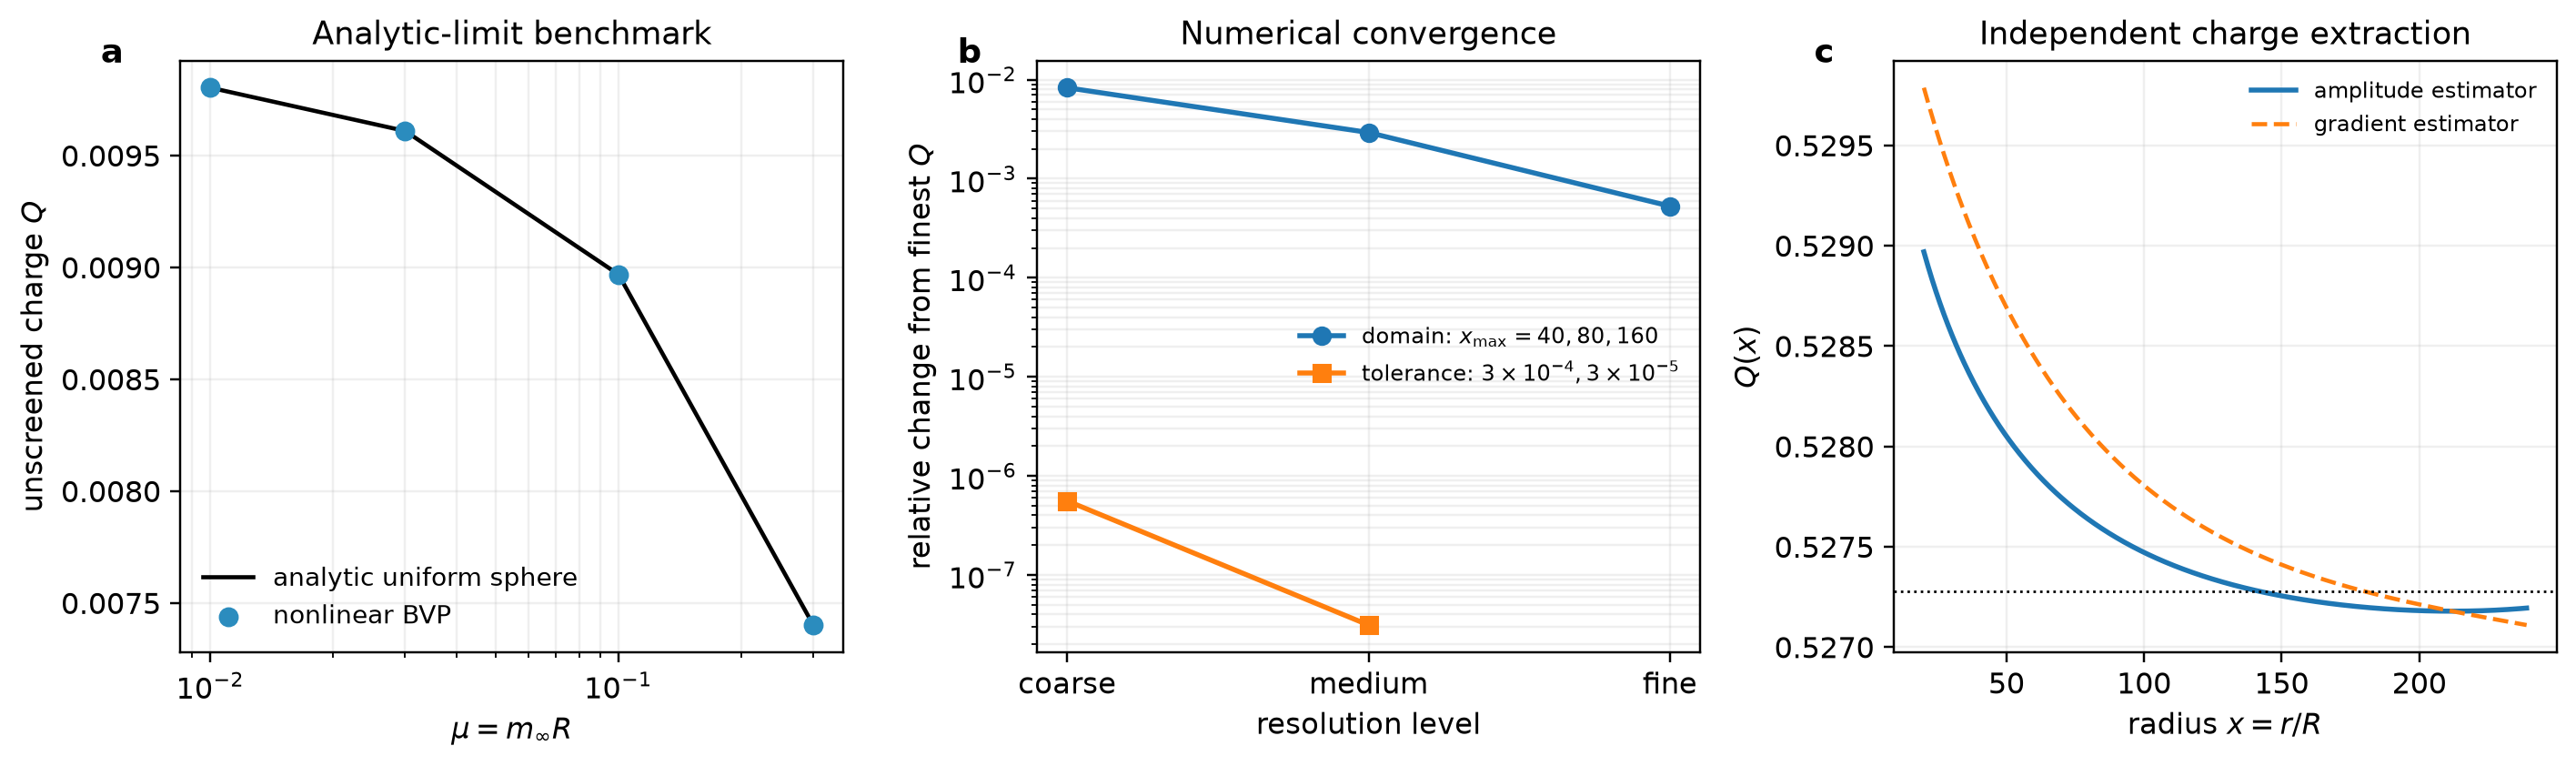
\includegraphics[width=\textwidth]{verification.png}
 \caption{Numerical verification. (a) The nonlinear BVP reproduces the known
 uniform-sphere Yukawa amplitude in the weak-source limit. (b) Outer-domain and
 collocation-tolerance convergence. (c) Independent exterior amplitude and
 gradient charge estimators approach the same plateau.}
 \label{fig:verification}
\end{figure}

\section{Results}

\subsection{Three screening regimes}

\Cref{fig:profiles} shows representative unscreened, transition, and screened
solutions.  The unscreened field varies throughout the source and has
$\qnum=0.885$.  The transition case has an interior close to its density
minimum but a visibly extended surface transition, with $\qnum=0.499$.  The
strongly screened source is almost frozen inside and has
$\qnum=5.47\times10^{-3}$.  In every case the two exterior charge estimators form
the same plateau, demonstrating that the plotted charge is measured from the
full solution rather than inserted through a thin-shell assumption.

\begin{figure}[H]
 \centering
 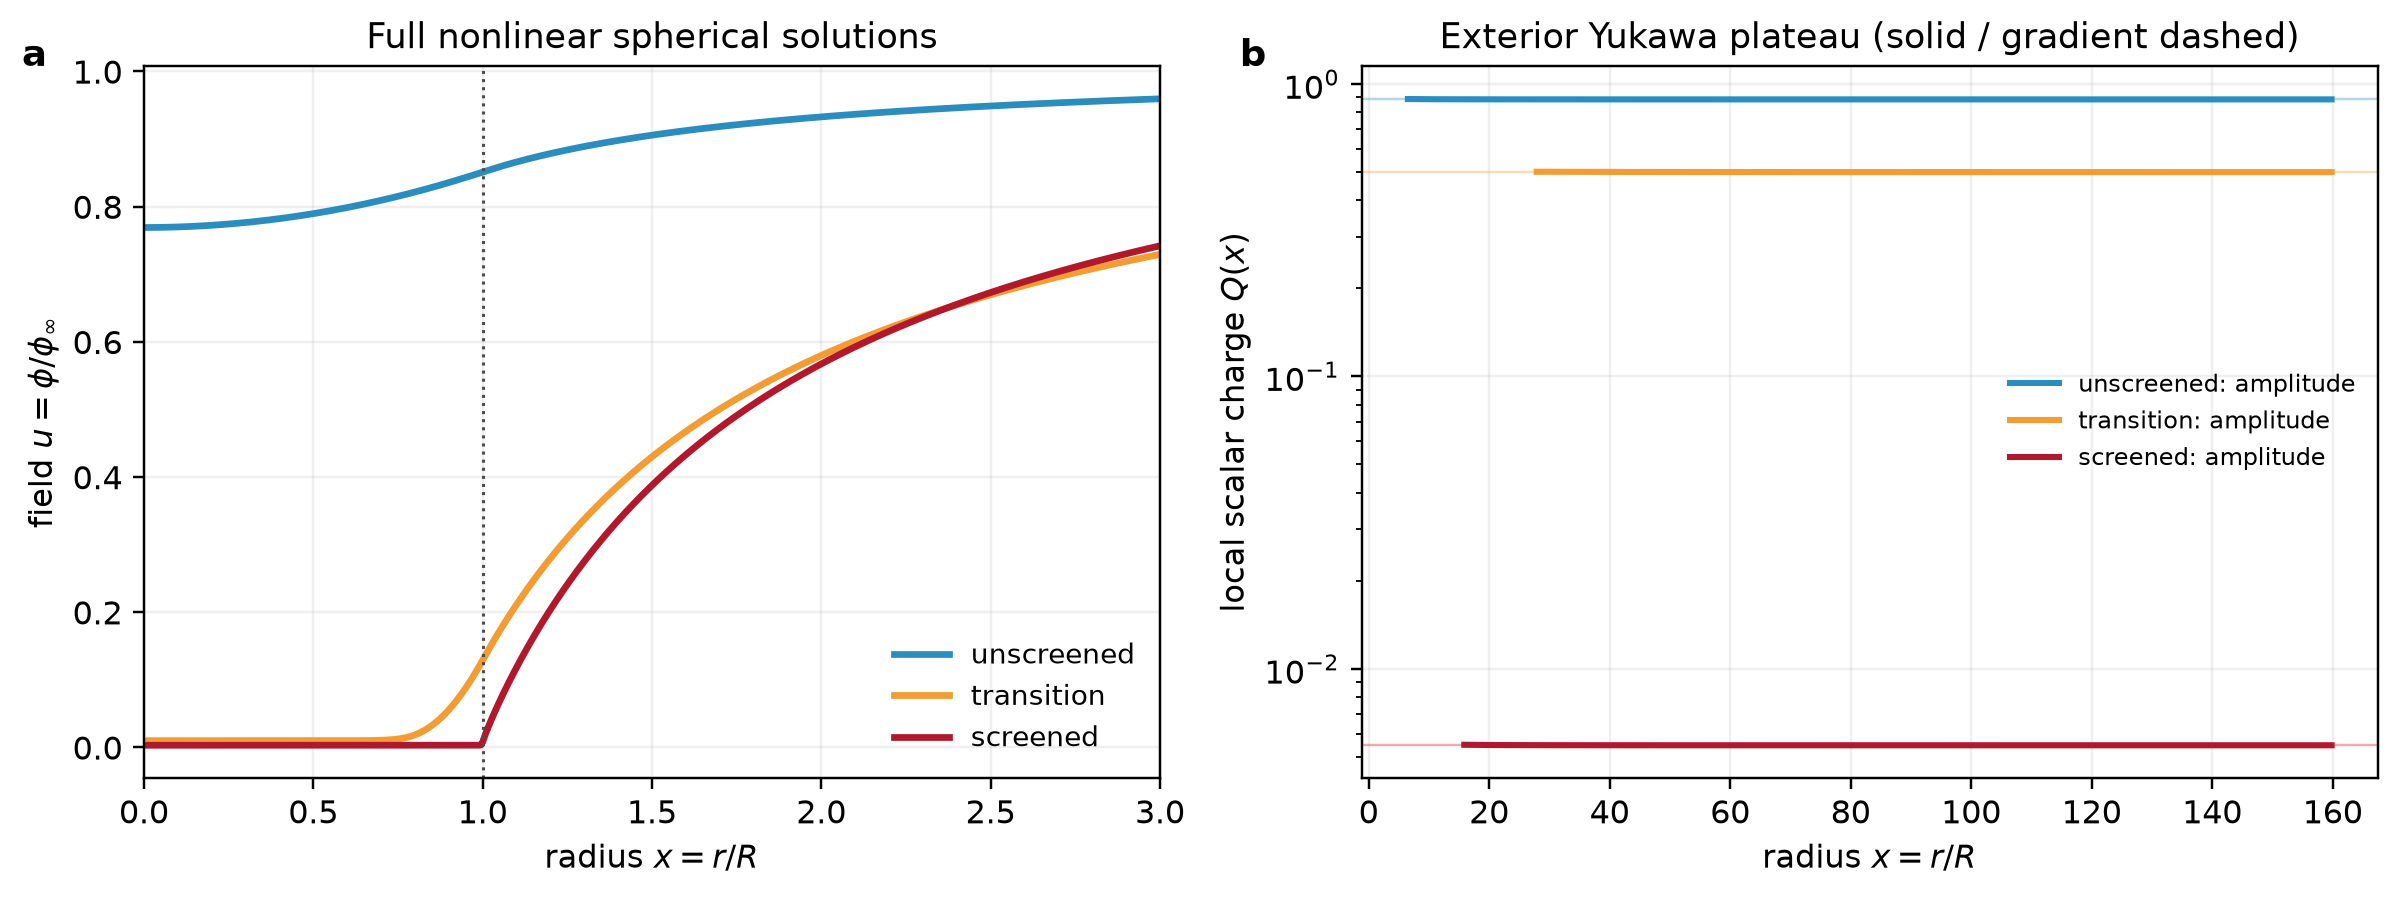
\includegraphics[width=0.86\textwidth]{profiles_and_charge_extraction.png}
 \caption{Full nonlinear field profiles and charge extraction.  The vertical
 dotted line marks the source surface.  Solid and dashed curves in the right
 panel are the amplitude and gradient estimators of
 \cref{eq:charge_estimators}.}
 \label{fig:profiles}
\end{figure}

\subsection{Accuracy atlas and failure conditions}

\Cref{fig:atlas} is the main approximation-validity result.  Color represents
the signed logarithmic error: red means the approximation overpredicts the
numerical charge.  The black curve is the 10\% error boundary.  The canonical
long-range charge, when continued from the surface, is accurate in the small-$\mu$
portion but fails in a broad transition band.  The center-point continuation is
often better but develops both positive and negative bias.  The active-shell
integral models the radial source distribution and removes most of the trend.

\begin{figure}[H]
 \centering
 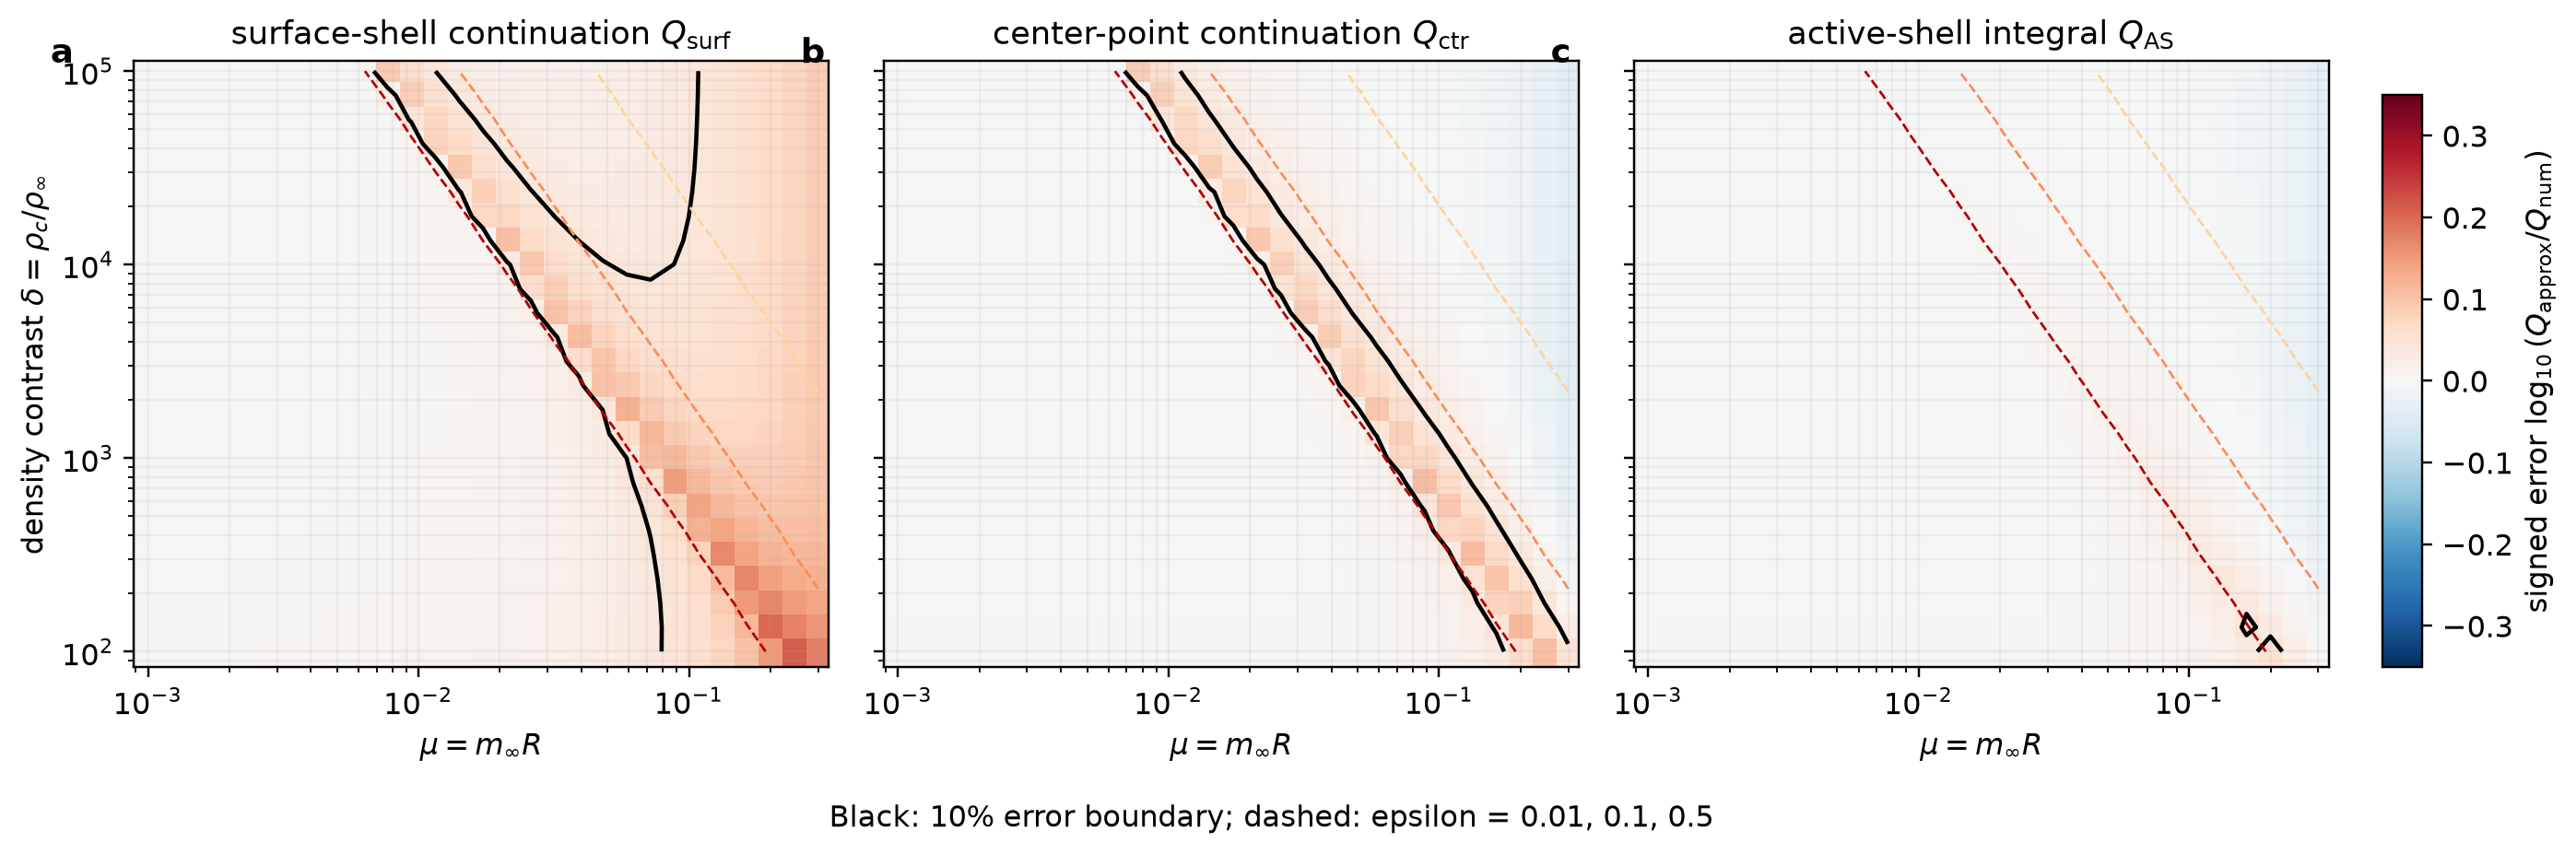
\includegraphics[width=\textwidth]{accuracy_atlas.png}
 \caption{Signed scalar-charge error for surface-shell and center-point
 continuations of the long-range law, and for the active-shell integral.  Black
 curves mark 10\% relative error; dashed curves show
 $\epsilon=0.01,0.1,0.5$.  Finite-$\mu$ continuation is not fixed by
 $\epsilon$ alone.}
 \label{fig:atlas}
\end{figure}

\begin{table}[H]
 \centering
 \caption{Error statistics over all 725 logarithmic grid points.}
 \label{tab:accuracy}
 \begin{tabular}{lrrrr}
  \toprule
  Approximation & Median error & 90th percentile & Maximum & Within 10\% \\
  \midrule
  Surface shell $\qsurf$ & 2.78\% & 23.0\% & 62.6\% & 68.8\% \\
  Center point $\qctr$ & 0.566\% & 8.89\% & 30.1\% & 91.3\% \\
  Finite shell only $\qms$ & 2.18\% & 18.0\% & 37.6\% & 77.5\% \\
  Active-shell integral $\qas$ & 0.391\% & 3.66\% & 13.1\% & 99.7\% \\
  \bottomrule
 \end{tabular}
\end{table}

The surface-shell continuation is larger than $\qnum$ at every sampled point.  Its
largest error, 62.6\%, occurs at $(\delta,\mu)=(100,0.245)$ with
$\epsilon=0.301$ and $m_cR=7.74$: neither the small-shell nor heavy-core
assumption is parametrically secure, and finite range is appreciable.  More
surprisingly, imposing only the familiar conditions $\epsilon<0.1$ and
$m_cR>10$ is insufficient: only 32.8\% of the 180 sampled points satisfying those
two conditions meet the 10\% target because $\mu$ can still be too large.  A
conservative filter selected from this grid is
\begin{equation}
 \boxed{\epsilon<0.1,\qquad m_cR>10,\qquad m_\infty R<0.035.}
 \label{eq:validity_gate}
\end{equation}
All 17 atlas points behind this filter are within 10\%, with an 8.09\% maximum
error.  I then test 12 logarithmic midpoint combinations excluded from the
atlas; all remain within 10\%, with an 8.15\% maximum.  This is an empirically
validated filter for the stated domain, not a universal theorem.  Its
significance is conceptual: a small shell and a heavy core do not by themselves
justify a finite-range continuation.

\Cref{fig:comparison} makes the separation quantitative.  The two naive
continuations bracket different parts of the grid.  The active-shell integral
follows the numerical diagonal closely; its two points outside 10\% lie in the
low-contrast, intermediate-screening corner, where a frozen-core shell ansatz
is least reliable.

\begin{figure}[H]
 \centering
 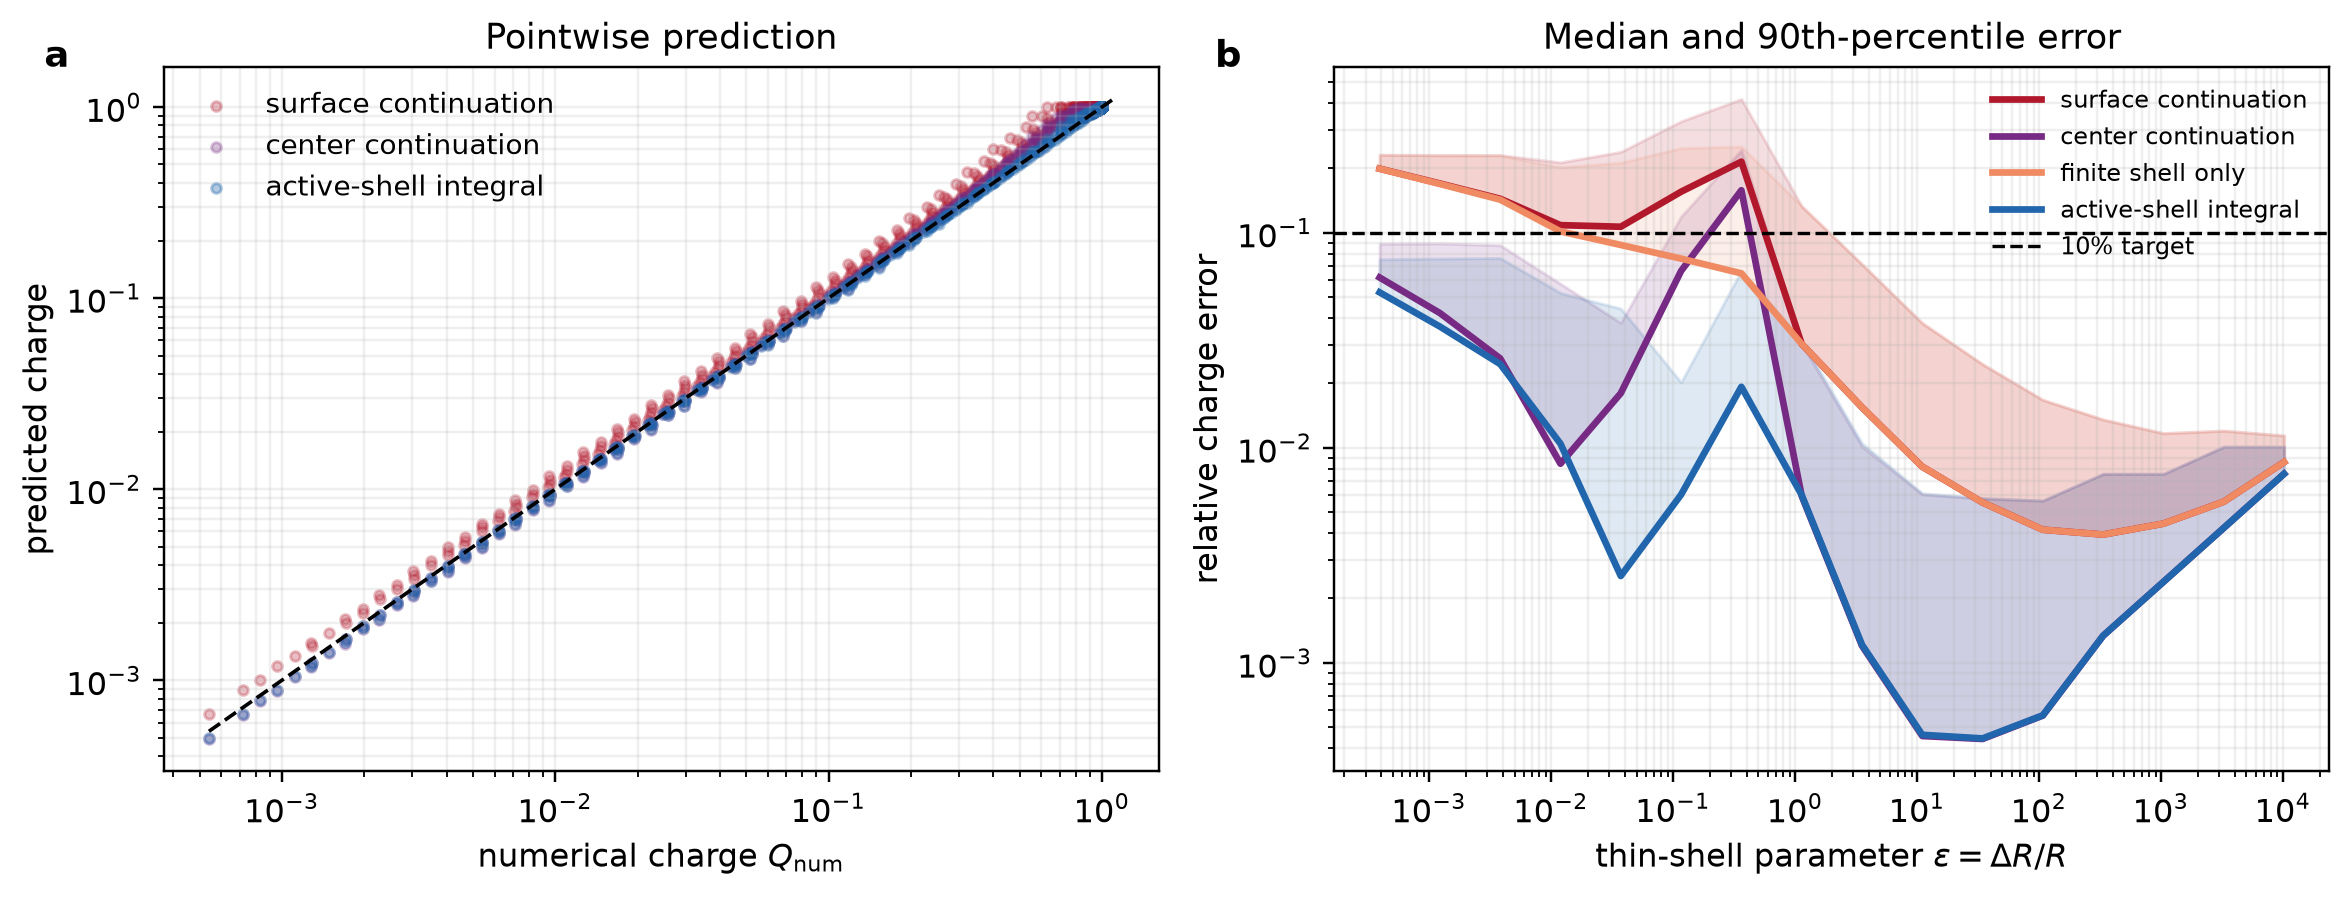
\includegraphics[width=\textwidth]{charge_comparison.png}
 \caption{Pointwise predictions and binned errors.  The filled bands in the
 right panel span the median to the 90th percentile within bins of $\epsilon$.
 The non-monotonic continuation error confirms that $\epsilon$ alone is not a
 complete validity variable.}
 \label{fig:comparison}
\end{figure}

\subsection{Illustrative force-ratio threshold map}

To propagate charge uncertainty into a dimensionless proxy decision, set
$\beta=1$, $Q_t=1$, and $x_p=1.5$ in \cref{eq:force_ratio}.  The left panel of
\cref{fig:detectability} shows $|a_5/a_N|$ for a hypothetical unscreened probe.
It is not an apparatus reach or discovery forecast: $(\delta,\mu)$ does not fix
the absolute Newtonian acceleration, and no detector noise, source scale, or
systematic uncertainty is included.

For a transparent stress test, choose
$\alpha_\star=|a_5/a_N|_\star=10^{-2}$.  A point is labeled ``above'' when its
predicted ratio exceeds this illustrative threshold.  The surface and center
continuations disagree at four grid points.  At every one of them the numerical
classification agrees with one continuation, so there is no
continuation-independent mismatch.  Among seven density rows with an in-grid
crossing, the median numerical-contour displacement is 0.032 dex for the
surface continuation and 0.0066 dex for the center continuation.  The third
panel shows the larger of the two naive-continuation errors in units of
$\alpha_\star$.

\begin{figure}[H]
 \centering
 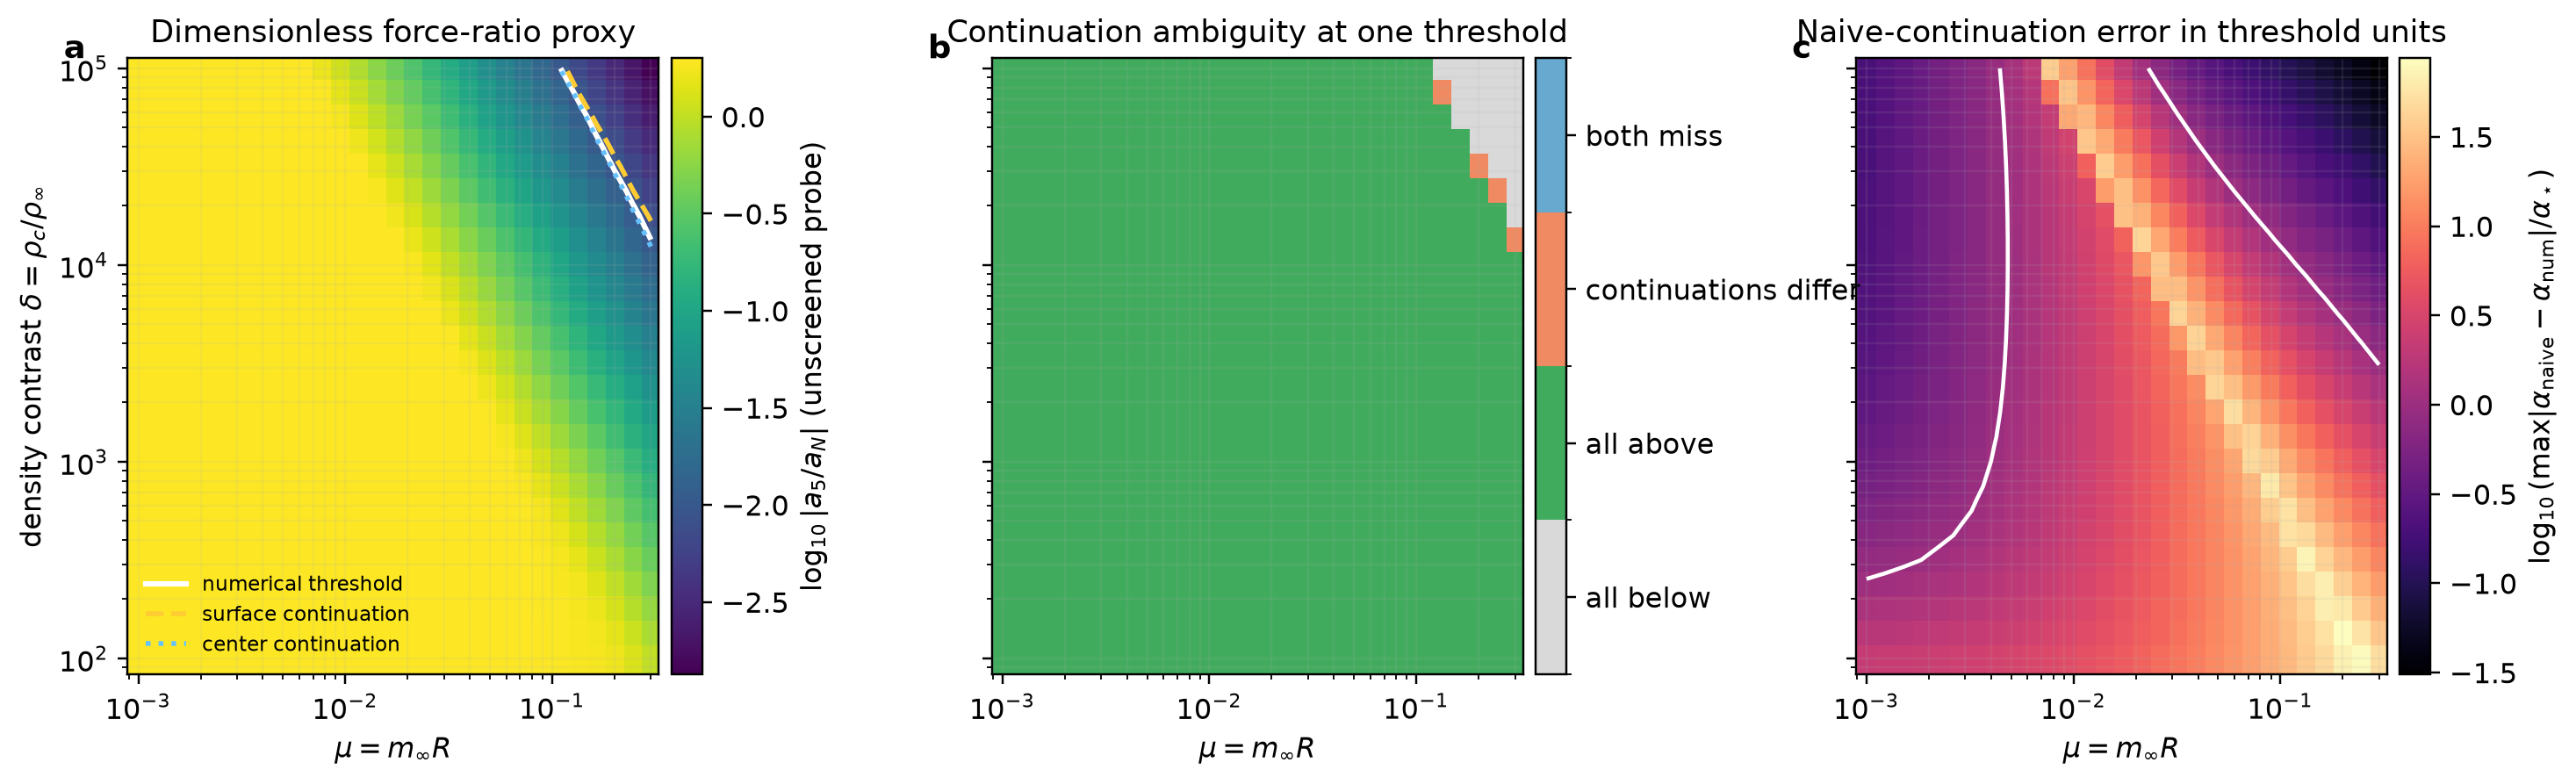
\includegraphics[width=\textwidth]{detectability_map.png}
 \caption{Accuracy-to-observability proxy. (a) Numerical fifth-force ratio for
 an unscreened probe, with numerical, surface-shell, and center-point threshold
 contours. (b) Points where the two finite-range continuations agree or differ.
 (c) The larger naive-continuation error in units of the illustrative threshold
 $\alpha_\star=10^{-2}$; the white contour marks unit error.}
 \label{fig:detectability}
\end{figure}

For a real past null experiment, the appropriate quantity would instead be a
reach ratio $\mathcal R=|a_5|/a_{\mathrm{lim}}$: $\mathcal R>1$ would mean that
the predicted signal exceeds the published limit only if geometry, signal
template, nuisance treatment, and confidence construction are matched; it does
not mean that a force was discovered.  For a future design one would use
$\mathcal D=|\Delta a_5|/\sigma_{\Delta a}$ and state the statistical and
systematic assumptions.  Atom-interferometer experiments
\cite{Hamilton2015,Sabulsky2019} and levitated bulk sensors \cite{Yin2022}
demonstrate that both probe types can be powerful despite very different
screening and noise mechanisms.

\section{Discussion}

\subsection{What the result adds}

The project now follows a conventional research logic.
\begin{description}[style=nextline]
 \item[Problem.] The long-range charge shortcut has no error bar through the
 screening transition and no unique finite-range continuation.
 \item[Proposed method.] Solve the nonlinear spherical BVP, measure an exterior
 charge without assuming a shell, compare two explicit continuations, and
 propagate their ambiguity into a threshold proxy.
 \item[Result.] Surface and center continuations differ substantially at finite
 range; an active-shell radial integral models most of the numerical trend.
 \item[Limited contribution.] The atlas supplies a held-out-checked validity
 filter, and \cref{eq:yukawa_matched} works at the 10\% level for 99.7\% of this
 grid.
\end{description}
The novelty is therefore not ``discovering screening'' and not claiming the
first thin-shell test.  It is the systematic connection between approximation
error and an observability proxy, together with a reproducible benchmark of an
active-shell ansatz built from the standard Yukawa radial integral.

\subsection{Relation to laboratory calculations}

Laboratory predictions contain additional layers absent here.  Chamber walls
can set the environmental field and change the force substantially; numerical
four-region studies have shown that geometry and walls matter
\cite{Schlogel2016}.  Elder et al.'s full three-dimensional calculation found
that the simple analytic prediction for a specific atom-interferometer geometry
was roughly 20\% high \cite{Elder2016}.  This establishes the direction of the
shift for that configuration only; walls and geometry can alter predictions in
either direction.  Those percentages are not directly comparable to
\cref{tab:accuracy}, because the present study isolates a single uniform sphere
and deliberately excludes chamber geometry.

The contemporary status of the underlying dark-energy model must also be
stated honestly.  Yin et al. report that their levitated force-sensor experiment
rules out the basic cosmologically viable chameleon model in the parameter
space they study \cite{Yin2022}.  The present calculation does not reopen that
claim.  It treats the $n=1$ chameleon as a clean nonlinear mechanics laboratory
for studying screening approximations and experimental-design bias.

\subsection{Limitations and next tests}

The conclusions are conditional on a static, isolated, uniform spherical
source; $n=1$; weak conformal coupling $D\rightarrow0$; and the sampled
$(\delta,\mu)$ range.  They do not include:
\begin{itemize}
 \item chamber walls, finite vacuum regions, source modulation, or nonspherical
 geometries;
 \item a numerical scalar charge for the test body or device-specific noise;
 \item other inverse-power indices, relativistic compactness, or time-dependent
 fields;
 \item a physical $(\Lambda,M_c)$ exclusion map.
\end{itemize}
A direct next project would solve a separate empty-chamber BVP to determine the
local environmental field, add source and wall regions, and compare atom and
bulk probes using their own $Q_t$ and $\sigma_a$.  Keeping the isolated-sphere
atlas separate is essential: otherwise intrinsic thin-shell error cannot be
distinguished from geometry error.

\section{Conclusion}

The long-range thin-shell approximation is useful, but ``$\epsilon$ is small''
does not define a unique finite-range prediction.  Across 725 nonlinear
spherical solutions, the surface-shell continuation is within 10\% at 68.8\%
of the grid and can overpredict by 62.6\%; the center-point continuation reaches
91.3\%.  The conservative filter $\epsilon<0.1$, $m_cR>10$, and
$m_\infty R<0.035$ succeeds on 17 atlas points and 12 held-out midpoints.  An
active-shell Yukawa integral reaches 10\% accuracy at 99.7\% of the grid, with a
0.39\% median error.  In a 14-point stratified $160\to240$ audit, the maximum
charge change is 0.056\% and no 10\%-accuracy classification flips.
At one illustrative threshold the two naive continuations disagree at four
points, while neither disagrees with the numerical result independently of
convention.  The scoped research result is therefore sharper than a claimed
experimental forecast: the active radial distribution, not $\epsilon$ alone,
controls how a screened source should be continued to finite range.

\appendix
\section{Reproducibility}
\begingroup\small

From the repository root, the complete scan, all figures, and metrics are
regenerated with
\begin{verbatim}
python -m Thin_Shell_Study.run_study --workers 4 --force
python -m unittest discover -v
\end{verbatim}
The principal files are:
\begin{itemize}
 \item \texttt{Thin\_Shell\_Study/thin\_shell\_model.py}: BVP and charge model;
 \item \texttt{Thin\_Shell\_Study/run\_study.py}: scan, verification, and plots;
 \item \texttt{Thin\_Shell\_Study/results/thin\_shell\_scan.csv}: all 725 points;
 \item \texttt{Thin\_Shell\_Study/results/gate\_validation\_midpoints.csv}: held-out filter checks;
 \item \texttt{Thin\_Shell\_Study/results/stratified\_domain\_audit.csv}: longer-domain spot checks;
 \item \texttt{Thin\_Shell\_Study/results/study\_metrics.json}: reported numbers;
 \item \texttt{tests/test\_thin\_shell\_study.py}: analytic and numerical tests.
\end{itemize}
The software environment used here is Python 3 with NumPy, SciPy, and
Matplotlib as listed in the repository's \texttt{requirements.txt}.
\endgroup

\clearpage
\begin{thebibliography}{99}

\bibitem{KhouryPRL}
J. Khoury and A. Weltman,
``Chameleon Fields: Awaiting Surprises for Tests of Gravity in Space,''
\emph{Phys. Rev. Lett.} \textbf{93}, 171104 (2004).
\href{https://doi.org/10.1103/PhysRevLett.93.171104}{doi:10.1103/PhysRevLett.93.171104}.

\bibitem{KhouryPRD}
J. Khoury and A. Weltman,
``Chameleon Cosmology,''
\emph{Phys. Rev. D} \textbf{69}, 044026 (2004).
\href{https://doi.org/10.1103/PhysRevD.69.044026}{doi:10.1103/PhysRevD.69.044026}.

\bibitem{TamakiTsujikawa}
T. Tamaki and S. Tsujikawa,
``Revisiting Chameleon Gravity: Thin-Shells and No-Shells with Appropriate Boundary Conditions,''
\emph{Phys. Rev. D} \textbf{78}, 084028 (2008).
\href{https://doi.org/10.1103/PhysRevD.78.084028}{doi:10.1103/PhysRevD.78.084028}.

\bibitem{BurrageSakstein}
C. Burrage and J. Sakstein,
``Tests of Chameleon Gravity,''
\emph{Living Rev. Relativ.} \textbf{21}, 1 (2018).
\href{https://doi.org/10.1007/s41114-018-0011-x}{doi:10.1007/s41114-018-0011-x}.

\bibitem{BurrageCopelandHinds}
C. Burrage, E. J. Copeland, and E. A. Hinds,
``Probing Dark Energy with Atom Interferometry,''
\emph{JCAP} \textbf{03}, 042 (2015).
\href{https://doi.org/10.1088/1475-7516/2015/03/042}{doi:10.1088/1475-7516/2015/03/042}.

\bibitem{Hamilton2015}
P. Hamilton et al.,
``Atom-Interferometry Constraints on Dark Energy,''
\emph{Science} \textbf{349}, 849--851 (2015).
\href{https://doi.org/10.1126/science.aaa8883}{doi:10.1126/science.aaa8883}.

\bibitem{Elder2016}
B. Elder et al.,
``Chameleon Dark Energy and Atom Interferometry,''
\emph{Phys. Rev. D} \textbf{94}, 044051 (2016).
\href{https://doi.org/10.1103/PhysRevD.94.044051}{doi:10.1103/PhysRevD.94.044051}.

\bibitem{Schlogel2016}
S. Schl\"ogel, S. Clesse, and A. F\"uzfa,
``Probing Modified Gravity with Atom Interferometry: A Numerical Approach,''
\emph{Phys. Rev. D} \textbf{93}, 104036 (2016).
\href{https://doi.org/10.1103/PhysRevD.93.104036}{doi:10.1103/PhysRevD.93.104036}.

\bibitem{Sabulsky2019}
D. O. Sabulsky et al.,
``Experiment to Detect Dark Energy Forces Using Atom Interferometry,''
\emph{Phys. Rev. Lett.} \textbf{123}, 061102 (2019).
\href{https://doi.org/10.1103/PhysRevLett.123.061102}{doi:10.1103/PhysRevLett.123.061102}.

\bibitem{Yin2022}
P. Yin et al.,
``Experiments with Levitated Force Sensor Challenge Theories of Dark Energy,''
\emph{Nature Phys.} \textbf{18}, 1181--1185 (2022).
\href{https://doi.org/10.1038/s41567-022-01706-9}{doi:10.1038/s41567-022-01706-9}.

\end{thebibliography}

\end{document}
